\documentclass[varwidth,border=0pt]{standalone}

% Tikz packages
\usepackage{tikz}
\usetikzlibrary{%
  patterns, plotmarks, backgrounds, shapes, arrows, calc, trees, positioning,
  chains, shapes.geometric, decorations.pathreplacing,
  decorations.pathmorphing, shapes.arrows, decorations.markings, quotes,
  arrows.meta, spy, fit, matrix
}

% General image and colour support
\usepackage{graphicx}
\usepackage{xcolor}

% Captions and subcaptions
\usepackage{caption}
\usepackage[labelformat=parens]{subcaption}
\renewcommand\thesubfigure{\sffamily\alph{subfigure})}

% Define main node type for networks
\tikzstyle{lnode2} = [%
  rectangle,
  rounded corners=5pt,
  draw=black,
  minimum height=0.65cm,
  align=center,
  fill=tbBlue,
  fill opacity=0.5,
  text opacity=1.0,
  text centered,
  text=black,
  inner sep=0.5pt,
  font=\tiny
]%
\tikzstyle{lnodeB} = [%
  rectangle,
  rounded corners=5pt,
  draw=white,
  minimum height=0.65cm,
  align=center,
  fill=white,
  fill opacity=1.0,
  text opacity=1.0,
  text centered,
  text=white,
  inner sep=0.5pt,
  font=\tiny
]%

% Define colour palette from (https://personal.sron.nl/~pault/#sec:qualitative)
\definecolor{tbBlue}{HTML}{0077BB}
\definecolor{tbCyan}{HTML}{33BBEE}
\definecolor{tbTeal}{HTML}{009988}
\definecolor{tbOrange}{HTML}{EE7733}
\definecolor{tbRed}{HTML}{CC3311}
\definecolor{tMagenta}{HTML}{EE3377}
\definecolor{tbGray}{HTML}{BBBBBB}

\begin{document}
  \begin{figure}
    \centering
    \begin{subfigure}[t]{0.5\textwidth}
      \caption{}
      \centering
      \sffamily
      \vspace*{-1.0em}
      \scalebox{0.75}{\begin{tikzpicture}[%
  cartoon/.style={%
    {Square[slant=-0.5,length=\the\pgflinewidth]}-{Stealth},
    line width=1.5pt
  },
  every node/.style={%
    %font=\sffamily\footnotesize\itshape,
    font=\sffamily\footnotesize,
    text=black,
    text centered,
    align=center
  },
  frame/.style={draw=black,inner sep=2pt}
]

  % Nodes
  \node[lnodeB] (A1) {L-Glutamate\\(1)};
  \node[below=1.0cm of A1] (P1) {};
  \node[lnodeB,text=black,right=1.5cm of P1,anchor=center] (A2) {L-Glutamyl 5-phosphate\\(2)};
  \node[lnodeB,below=1.0cm of P1] (A3) {L-Glutamate 5-semialdehyde\\(3)};
  \node[below=1.0cm of A3] (P2) {};
  \node[lnodeB,left=1.5cm of P2,anchor=center] (A4) {(S)-1-Pyrroline-5-carboxylate\\(4)};
  \node[lnodeB,right=1.5cm of P2,anchor=center] (A5) {L-Ornithine\\(5)};
  \node[lnodeB,below=1.0cm of P2] (A6) {L-Proline\\(6)};
  \node[above=0.5cm of A1] (Y1) {};
  \node[below=0.5cm of A6] (Y2) {};

  % Intra-node edges
  \draw[postaction={decorate},cartoon] (A1) to [bend right=45] node [left=0.1pt,yshift=-0pt] {2} (A3);
  \draw[cartoon] (A1.center) to node [above right=0.1pt,yshift=-5pt,xshift=+6pt] {2} (A2);
  \draw[cartoon] (A2.center) to node [below right=0.1pt,xshift=-5pt] {2} (A3);
  \draw[cartoon] (A3.center) to node [above left=0.1pt,yshift=-5pt,xshift=-6pt] {2} (A4);
  \draw[cartoon] (A3.center) to node [above right=0.1pt,yshift=-5pt,xshift=+6pt] {2} (A5);
  \draw[cartoon] (A4.center) to node [below left=0.1pt,xshift=+5pt] {2} (A6);
  \draw[cartoon] (A5.center) to node [below right=0.1pt,xshift=-5pt] {2} (A6);

  % Boundary edges
  \draw[cartoon] (Y1.center) to node [left,yshift=5pt] {4} (A1.north);
  \draw[cartoon] (A6.center) to node [left] {4} (Y2.center);

  % Nodes
  \node[lnodeB] (A1) {L-Glutamate\\(1)};
  \node[below=1.0cm of A1] (P1) {};
  \node[lnodeB,text=black,right=1.5cm of P1,anchor=center] (A2) {L-Glutamyl 5-phosphate\\(2)};
  \node[lnodeB,below=1.0cm of P1] (A3) {L-Glutamate 5-semialdehyde\\(3)};
  \node[below=1.0cm of A3] (P2) {};
  \node[lnodeB,left=1.5cm of P2,anchor=center] (A4) {(S)-1-Pyrroline-5-carboxylate\\(4)};
  \node[lnodeB,right=1.5cm of P2,anchor=center] (A5) {L-Ornithine\\(5)};
  \node[lnodeB,below=1.0cm of P2] (A6) {L-Proline\\(6)};
  \node[above=0.5cm of A1] (Y1) {};
  \node[below=0.5cm of A6] (Y2) {};

  \node[lnode2] (A1) {L-Glutamate\\(1)};
  \node[lnode2,right=1.5cm of P1,anchor=center] (A2) {L-Glutamyl 5-phosphate\\(2)};
  \node[lnode2,below=1.0cm of P1] (A3) {L-Glutamate 5-semialdehyde\\(3)};
  \node[lnode2,left=1.5cm of P2,anchor=center] (A4) {(S)-1-Pyrroline-5-carboxylate\\(4)};
  \node[lnode2,right=1.5cm of P2,anchor=center] (A5) {L-Ornithine\\(5)};
  \node[lnode2,below=1.0cm of P2] (A6) {L-Proline\\(6)};
  \node[rectangle,width=0.1cm,fill=white,above=0.60cm of A1] (Z) {};

\end{tikzpicture}

}\\  %https://www.kegg.jp/pathway/rn00330
      \vspace*{-0.5em}
      \scalebox{0.75}{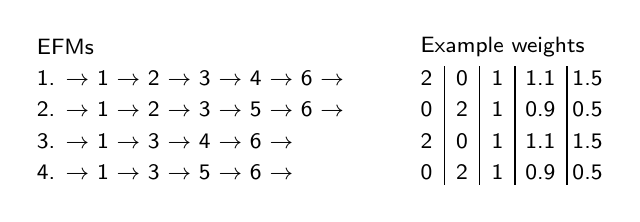
\begin{tikzpicture}[%
    >=latex,
    decoration={%
      markings,
      mark=at position 1.0 with {\arrow{>}}
    },
    every node/.style={%
      font=\sffamily\footnotesize\itshape,
      text=gray,
      text centered,
      align=center
    },
    frame/.style={draw=black,inner sep=2pt}
  ]

  \node[black, font=\sffamily\footnotesize] (t1) {EFMs};
  \node[black, font=\sffamily\footnotesize, below=0.4cm of t1.west, anchor=west]
    (t2)
    {1. $\rightarrow$ 1 $\rightarrow$ 2 $\rightarrow$ 3 $\rightarrow$ 4 $\rightarrow$ 6 $\rightarrow$};
  \node[black, font=\sffamily\footnotesize, below=0.4cm of t2.west, anchor=west]
    (t3)
    {2. $\rightarrow$ 1 $\rightarrow$ 2 $\rightarrow$ 3 $\rightarrow$ 5 $\rightarrow$ 6 $\rightarrow$};
  \node[black, font=\sffamily\footnotesize, below=0.4cm of t3.west, anchor=west]
    (t4)
    {3. $\rightarrow$ 1 $\rightarrow$ 3 $\rightarrow$ 4 $\rightarrow$ 6 $\rightarrow$};
  \node[black, font=\sffamily\footnotesize, below=0.4cm of t4.west, anchor=west]
    (t5)
    {4. $\rightarrow$ 1 $\rightarrow$ 3 $\rightarrow$ 5 $\rightarrow$ 6 $\rightarrow$};

  \node[black, font=\sffamily\footnotesize, right=3.9cm of t1] (u1) {Example weights\textcolor{white}{ss}};
  \node[black, font=\sffamily\footnotesize, below=0.4cm of u1, anchor=south]
    (u2)
    {\textcolor{white}{Example weightsss}};
  \node[black, font=\sffamily\footnotesize, below=0.4cm of u2, anchor=south]
    (u3)
    {\textcolor{white}{Example weightsss}};
  \node[black, font=\sffamily\footnotesize, below=0.4cm of u3, anchor=south]
    (u4)
    {\textcolor{white}{Example weightsss}};
  \node[black, font=\sffamily\footnotesize, below=0.4cm of u1.west, anchor=west]
    (a1)
    {2};
  \node[black, font=\sffamily\footnotesize, below=0.4cm of u1.west, anchor=west,xshift=0.45cm]
    (a2)
    {0};
  \node[black, font=\sffamily\footnotesize, below=0.4cm of u1.west, anchor=west,xshift=0.9cm]
    (a3)
    {1};
  \node[black, font=\sffamily\footnotesize, below=0.4cm of u1.east, anchor=east,xshift=-0.6cm]
    (a4)
    {1.1};
  \node[black, font=\sffamily\footnotesize, below=0.4cm of u1.east, anchor=east,xshift=0cm]
    ()
    {1.5};

  \node[black, font=\sffamily\footnotesize, below=0.4cm of u2.west, anchor=west]
    ()
    {0};
  \node[black, font=\sffamily\footnotesize, below=0.4cm of u2.west, anchor=west,xshift=0.45cm] ()
    {2};
  \node[black, font=\sffamily\footnotesize, below=0.4cm of u2.west, anchor=west,xshift=0.9cm]
    ()
    {1};
  \node[black, font=\sffamily\footnotesize, below=0.4cm of u2.east, anchor=east,xshift=-0.6cm]
    ()
    {0.9};
  \node[black, font=\sffamily\footnotesize, below=0.4cm of u2.east, anchor=east,xshift=0cm]
    ()
    {0.5};
  \node[black, font=\sffamily\footnotesize, below=0.4cm of u3.west, anchor=west]
    ()
    {2};
  \node[black, font=\sffamily\footnotesize, below=0.4cm of u3.west, anchor=west,xshift=0.45cm]
    ()
    {0};
  \node[black, font=\sffamily\footnotesize, below=0.4cm of u3.west, anchor=west,xshift=0.9cm]
    ()
    {1};
  \node[black, font=\sffamily\footnotesize, below=0.4cm of u3.east, anchor=east,xshift=-0.6cm]
    ()
    {1.1};
  \node[black, font=\sffamily\footnotesize, below=0.4cm of u3.east, anchor=east,xshift=0cm]
    ()
    {1.5};

  \node[black, font=\sffamily\footnotesize, below=0.4cm of u4.west, anchor=west]
    (b1)
    {0};
  \node[black, font=\sffamily\footnotesize, below=0.4cm of u4.west, anchor=west,xshift=0.45cm]
    (b2)
    {2};
  \node[black, font=\sffamily\footnotesize, below=0.4cm of u4.west, anchor=west,xshift=0.9cm]
    (b3)
    {1};
  \node[black, font=\sffamily\footnotesize, below=0.4cm of u4.east, anchor=east,xshift=-0.6cm]
    (b4)
    {0.9};
  \node[black, font=\sffamily\footnotesize, below=0.4cm of u4.east, anchor=east,xshift=0cm]
    ()
    {0.5};

  % Vertical bars
  \node[black, right=0.1cm of a1, xshift=-2.0mm,yshift=+1.5mm] (l1) {};
  \node[black, right=0.1cm of b1, xshift=-2.0mm,yshift=-1.5mm] (m1) {};
  \draw[black] (l1.center) to (m1.center);
  \node[black, right=0.1cm of a2, xshift=-2.0mm,yshift=+1.5mm] (l2) {};
  \node[black, right=0.1cm of b2, xshift=-2.0mm,yshift=-1.5mm] (m2) {};
  \draw[black] (l2.center) to (m2.center);
  \node[black, right=0.1cm of a3, xshift=-2.0mm,yshift=+1.5mm] (l3) {};
  \node[black, right=0.1cm of b3, xshift=-2.0mm,yshift=-1.5mm] (m3) {};
  \draw[black] (l3.center) to (m3.center);
  \node[black, right=0.1cm of a4, xshift=-2.0mm,yshift=+1.5mm] (l4) {};
  \node[black, right=0.1cm of b4, xshift=-2.0mm,yshift=-1.5mm] (m4) {};
  \draw[black] (l4.center) to (m4.center);


\end{tikzpicture}

}
    \end{subfigure}\hfill%
    \begin{subfigure}[t]{0.5\textwidth}
      \caption{}
      \centering
      \sffamily
      \vspace*{-1.0em}
      \scalebox{0.75}{\begin{tikzpicture}[%
  cartoon/.style={%
    {Square[slant=-0.5,length=\the\pgflinewidth]}-{Stealth},
    line width=1.5pt
  },
  every node/.style={%
    %font=\sffamily\footnotesize\itshape,
    font=\sffamily\footnotesize,
    text=black,
    text centered,
    align=center
  },
  frame/.style={draw=black,inner sep=2pt}
]

  % Nodes
  \node[lnodeB] (A1) {5,6,7,8-Tetrahydrofolate (THF)\\(1)};
  \node[below=1.0cm of A1] (P1) {};
  \node[lnodeB,left=1.0cm of P1,xshift=1.13cm,anchor=center] (A2) {10-Formyl-THF\\(2)};
  \node[lnodeB,below=1.0cm of P1] (A3) {5,10-Methenyl-THF\\(3)};
  \node[below=1.0cm of A4] (P2) {};
  \node[lnode2,below=1.13cm of A3,anchor=center] (A6) {5,10-Methylene-THF\\(6)};
  \node (P3) at ($(A3)!0.5!(A6)$) {};
  \node[lnodeB,left=1.25cm of P3] (A4) {5-Formimino-THF\\(4)};
  \node[lnodeB,right=1.25cm of P3] (A5) {5-Formyl-THF\\(5)};
  \node[lnodeB,below=1.12cm of A6,anchor=center] (A7) {5-Methyl-THFO\\(7)};
  \node[left=0.1cm of A4] (X1) {};
  \node[left=0.3cm of A4] (X2) {};
  \node[right=0.1cm of A5,yshift=1.0cm] (X3) {};
  \node[right=0.3cm of A5,yshift=1.0cm] (X4) {};
  \node[above=0.5cm of A1] (Y1) {};
  \node[below=0.5cm of A7] (Y2) {};

  % Intra-node edges
  \draw[postaction={decorate},cartoon] (A1.center) to [bend right=40] node [below right=0.1pt,yshift=-0pt] {3} (A2);
  \draw[postaction={decorate},cartoon] (A2.center) to [bend right=40] node [below left=0.1pt,yshift=+12.4pt] {2} (A1);
  \draw[postaction={decorate},cartoon] (A2.center) to [bend right=40] node [below right=0.1pt,yshift=-0pt] {3} (A3);
  \draw[postaction={decorate},cartoon] (A3.center) to [bend right=40] node [below left=0.1pt,yshift=+12pt] {2} (A2);
  \draw[postaction={decorate},cartoon,draw=tbGray] ([xshift=0.4cm]A3.center) to [bend right=40] node [right=0.1pt,yshift=-2pt] {} (A5);
  \draw[postaction={decorate},cartoon,draw=tbGray] ([xshift=-0.1cm]A5.center) to [bend right=40] node [left=0.1pt,yshift=+2pt] {} ([yshift=0.2cm]A3.east);
  \draw[postaction={decorate},cartoon] (A3.center) to [bend right=40] node [below=0.1pt,yshift=-0pt] {2} ([xshift=0.1cm]A4.north);
  \draw[postaction={decorate},cartoon] (A4.center) to [bend right=40] node [above=0.1pt,xshift=+3pt] {3} ([xshift=-0.4cm]A3.south);
  \draw[postaction={decorate},cartoon,draw=tbGray] (A3.center) to [bend right=40] node [right=0.1pt,yshift=-2pt] {} (A6);
  \draw[postaction={decorate},cartoon,draw=tbGray] (A6.center) to [bend right=40] node [left=0.1pt,yshift=+2pt] {} (A3);
  \draw[postaction={decorate},cartoon,draw=tbGray] (A6.center) to node [right=0.1pt,yshift=-2pt] {} (A7);

  \draw[cartoon,rounded corners=15pt] ([xshift=-0.4cm]A3.center) to [bend left=40] node [left=0.1pt] {3\qquad 2\qquad 2} ([xshift=-0.4cm]A1.south);
  \draw[cartoon,rounded corners=15pt] (A4.center) |- ([yshift=-0.25cm]A1.west);
  \draw[cartoon,rounded corners=15pt] ([yshift=-0.05cm]A1.center) -| ([xshift=-0.2cm]A4.north);
  \draw[cartoon,rounded corners=15pt,draw=tbGray] ([xshift=-0.1cm]A5.center) |- (A2.east);
  \draw[cartoon,rounded corners=15pt,draw=tbGray] (A5.center) |- ([yshift=-0.25cm]A1.east);
  \draw[cartoon,rounded corners=15pt,draw=tbGray] ([yshift=+0.025cm]A1.center) -| (X1.center) |- ([yshift=0.4cm]A7);
  \draw[cartoon,rounded corners=15pt,draw=tbGray] ([yshift=-0.1cm]A7.center) -| (X2.center) |- ([yshift=0.55cm]A1);
  \draw[cartoon,rounded corners=15pt,draw=tbGray] ([yshift=+0.025cm]A1.center) -| (X3.center) |- ([yshift=0.4cm]A6);
  \draw[cartoon,rounded corners=15pt,draw=tbGray] ([yshift=-0.1cm]A6.center) -| (X4.center) |- ([yshift=0.5cm]A1);

  % Boundary edges
  \draw[cartoon,tbGray] (Y1.center) to node [left,yshift=5pt] {} (A1.north);
  \draw[cartoon,tbGray] (A7.center) to node [left] {} (Y2.center);

  % Nodes
  \node[lnodeB] (A1) {5,6,7,8-Tetrahydrofolate (THF)\\(1)};
  \node[below=1.0cm of A1] (P1) {};
  \node[lnodeB,text=black,left=1.0cm of P1,xshift=1.13cm,anchor=center] (A2) {10-Formyl-THF\\(2)};
  \node[lnodeB,below=1.0cm of P1] (A3) {5,10-Methenyl-THF\\(3)};
  \node[below=1.0cm of A3] (P2) {};
  \node (P3) at ($(A3)!0.5!(A6)$) {};
  \node[lnodeB,left=1.25cm of P3] (A4) {5-Formimino-THF\\(4)};
  \node[lnodeB,right=1.25cm of P3,draw=tbGray,text=tbGray] (A5) {5-Formyl-THF\\(5)};
  \node[lnodeB,below=1.12cm of A6,anchor=center,draw=tbGray,text=tbGray] (A7) {5-Methyl-THFO\\(7)};
  \node[lnodeB,below=1.13cm of A3,anchor=center,draw=tbGray,text=tbGray] (A6) {5,10-Methylene-THF\\(6)};

  % Nodes
  \node[lnode2] (A1) {5,6,7,8-Tetrahydrofolate (THF)\\(1)};
  \node[lnode2,text=black,left=1.0cm of P1,xshift=1.13cm,anchor=center] (A2) {10-Formyl-THF\\(2)};
  \node[lnode2,below=1.0cm of P1] (A3) {5,10-Methenyl-THF\\(3)};
  \node[lnode2,below=1.13cm of A3,anchor=center,draw=black,text=black,text opacity=0.5,fill opacity=0.25,draw opacity=0.5] (A6) {5,10-Methylene-THF\\(6)};
  \node[lnode2,left=1.25cm of P3] (A4) {5-Formimino-THF\\(4)};
  \node[lnode2,right=1.25cm of P3,draw=black,text=black,text opacity=0.5,fill opacity=0.25,draw opacity=0.5] (A5) {5-Formyl-THF\\(5)};
  \node[lnode2,below=1.12cm of A6,anchor=center,draw=black,text=black,text opacity=0.5,fill opacity=0.25,draw opacity=0.5] (A7) {5-Methyl-THFO\\(7)};

  \node[rectangle,width=0.1cm,fill=white,above=0.60cm of A1] (Z) {};

\end{tikzpicture}


}\\ % https://www.genome.jp/pathway/map00670
      \vspace*{-0.5em}
      \scalebox{0.75}{\input{input-example-2-efms.tex}}
    \end{subfigure}
  \end{figure}
\end{document}

